\documentclass[a4paper,12pt]{article}
\author{Grunda}
\usepackage[utf8]{inputenc}   
\usepackage[T2A]{fontenc}     % Для кириличних шрифтів
\usepackage[ukrainian]{babel} % Для української мови
\usepackage{geometry}         % Для настройки полів
\usepackage{amsmath}          % Для математичних формул
\usepackage{amsfonts}         % Для шрифтів математичних символів
\usepackage{amssymb}          % Для математичних символів
\usepackage{graphicx}         % Для вставки зображень (якщо потрібно)
\usepackage{hyperref}         % Для створення гіперпосилань у змісті
\usepackage{booktabs} % Для улучшенных линий в таблицах
\usepackage{caption}  % Для управления подписями таблиц
\usepackage{adjustbox} % Для изменения размера таблицы
\usepackage{subcaption} % Для подписи подрисунков


\geometry{left=2.5cm, right=2.5cm, top=2.5cm, bottom=2.5cm}

\title{Звіт до лабораторної роботи}
\author{Ярослав Грунда \\ Фі-21, ФТІ КПІ}
\date{\today}

\begin{document}

\maketitle

\tableofcontents 
\newpage

\section{Мета роботи}
Реалізувати алгоритми пошуку шляхів найменшої ваги від заданої вершини до усіх інших вершин: 
алгоритм Дейкстри та алгоритм Беллмана-Форда; порівняти їх між собою.

\section{Алгоритм Дейкстри}

\subsection{Опис роботи алгоритму Дейкстри}
Алгоритм Дейкстри шукає найкоротші шляхи від стартової вершини до всіх інших у графі з невід'ємними вагами.

\textbf{Ініціалізація:}

Відстані до всіх вершин — $\infty$, до стартової вершини — $0$.  
Попередники для відновлення шляху ініціалізуються як None.  
Використовується масив для позначення відвіданих вершин.  

\textbf{Основний цикл:}

Оновлюються відстані для сусідів поточної вершини. Якщо нова відстань коротша, оновлюється значення та попередник.  
Вершина позначається як відвідана.  
Наступна вершина вибирається серед невідвіданих із найменшою відстанню.  

\textbf{Завершення:}

Алгоритм завершується, коли оброблено всі доступні вершини.

\subsection{Особливості алгоритму Дейкстри}
Для представлення графа у вигляді списків суміжності:

У найпростішому випадку, коли для пошуку вершини з мінімальною відстанню проглядаються всі вершини, тобто використовується лінійний пошук, складність алгоритму зростає до $O(V^2 + E)$, оскільки:

\begin{itemize}
    \item Щоб вибрати наступну вершину, ми переглядаємо всі невідвідані вершини. Цей процес займає $O(V)$ часу для кожної вершини.
    \item Оскільки цей пошук виконується для кожної з $V$ вершин, загальна складність для цього пошуку — $O(V^2)$.
    \item Для кожної вершини алгоритм перевіряє всі її сусіди (ребра) і оновлює відстані. Оновлення сусідів виконується за $O(E)$, де $E$ — кількість ребер.
\end{itemize}

Якщо використовувати чергу з пріоритетом, де операції вилучення та додавання елементів дорівнюють $O(\log V)$, то складність алгоритму зменшується і становить $O((V + E) \log V)$, оскільки:

\begin{itemize}
    \item Кожну вершину обробляємо один раз, додаючи її в чергу. Для всіх $V$ вершин це дає $O(V \log V)$.
    \item Для кожного ребра ми можемо виконати оновлення відстані, що супроводжується з додаванням до черги ребра. Для всіх $E$ ребер це дає $O(E \log V)$.
\end{itemize}

Для представлення графа у вигляді матриці суміжності:

Алгоритм Дейкстри не є ефективним, оскільки замість того, щоб проглядати тільки існуючі ребра, ми проглядаємо всі можливі ребра: $O(V^2 + V^2)$ для лінійного пошуку, $O(V^2 + E \log V)$ 
з використанням пріоритетної черги.

\section{Алгоритм Беллмана-Форда}

\subsection{Опис роботи алгоритму Беллмана-Форда}
Алгоритм Беллмана-Форда — це метод для знаходження найменших відстаней від однієї вершини (стартової) до всіх інших вершин у графі. 
Він працює навіть у випадках, коли граф може містити ребра з від'ємними вагами, проте не допускає наявності від'ємних циклів.

\textbf{Ініціалізація:}

Створюється словник \texttt{distances}, у якому для кожної вершини зберігається відстань від стартової вершини. Усі значення ініціалізуються значенням $\infty$ (нескінченність), 
окрім стартової вершини, для якої відстань дорівнює $0$.  
Ініціалізується словник \texttt{previous}, у якому для кожної вершини зберігається попередник на найкоротшому шляху.

\textbf{Основний цикл:}

Алгоритм виконує $n-1$ ітерацій (де $n$ — кількість вершин у графі). На кожній ітерації:
\begin{itemize}
    \item Для кожної вершини у графі перевіряються всі сусіди.
    \item Якщо нова обчислена відстань до сусіда менша за вже відому, то відстань оновлюється, а також оновлюється попередник для цього сусіда.
\end{itemize}

\textbf{Перевірка на від'ємні цикли:}

Після основного циклу алгоритм перевіряє наявність від'ємних циклів. Якщо є можливість ще зменшити відстань до якоїсь вершини, це означає, що граф містить від'ємний цикл.

\subsection{Особливості алгоритму Беллмана-Форда}
Складність для представлення у вигляді списків суміжності: $O(V \cdot E)$ - алгоритм проходить по всіх ребрах $n-1$ разів.  
У вигляді матриці суміжності: $O(V^3)$ - алгоритм проходить по всіх можливих ребрах, навіть якщо вони не існують.

\section{Гіпотези}
1. Алгоритми Дейкстри з лінійним пошуком працює повільніше ніж з використанням пріоритетної черги.
2. Алгоритми Дейкстри та Беллмана-Форда працюють швидше при представленні списками щільності ніж при представленні матрицею не зважаючи на щільність.
3. Алгоритми Дейкстри та Беллмана-Форда працюють швидше при зменшені щільності графа для представлення списками суміжності. (Дейкстра з Чергою)
4. Алгоритм Дейкстри працює швидше за алгоритм Беллмана-Форда при будь-якому представленні та щільності.

\section{Таблички порівняння}

\begin{table}[ht]
    \centering
    \caption{Час виконання алгоритмів для щільності 0.7 (в мікросекундах)}
    \adjustbox{max width=\textwidth}{ 
        \begin{tabular}{@{}lcccccccccccccc@{}}
            \toprule
            num vertices & \texttt{dijkstra} & \texttt{dijkstra\_h} & \texttt{dijkstra\_m} & \texttt{dijkstra\_mh} & \texttt{bellman\_ford} & \texttt{bellman\_ford\_matrix} \\ 
            \midrule
            5   & 39.96     & 0.0           & 0.0           & 0.0           & 20.00     & 40.67 \\ 
            25  & 59.37     & 0.0           & 59.10         & 20.02        & 1606.00   & 3845.00 \\ 
            45  & 344.30    & 39.83         & 915.50        & 402.00       & 9020.00   & 23770.00 \\ 
            65  & 636.60    & 586.60        & 813.00        & 705.00       & 19700.00  & 75170.00 \\ 
            85  & 1238.00   & 482.60        & 1484.00       & 2460.00      & 55310.00  & 179300.00 \\ 
            105 & 1494.00   & 986.70        & 2705.00       & 3386.00      & 110800.00 & 351800.00 \\ 
            125 & 2392.00   & 1023.00       & 3791.00       & 4179.00      & 170800.00 & 548300.00 \\ 
            145 & 3262.00   & 2309.00       & 4991.00       & 4909.00      & 277800.00 & 895400.00 \\ 
            165 & 3750.00   & 1783.00       & 5911.00       & 6723.00      & 367700.00 & 1199000.00 \\ 
            185 & 4048.00   & 1988.00       & 7121.00       & 8326.00      & 539700.00 & 1697000.00 \\ 
            205 & 5801.00   & 3062.00       & 8995.00       & 9847.00      & 739700.00 & 2335000.00 \\ 
            225 & 7925.00   & 3619.00       & 12590.00      & 13400.00     & 1059000.00 & 3115000.00 \\ 
            245 & 7914.00   & 3735.00       & 11920.00      & 14070.00     & 1214000.00 & 3738000.00 \\ 
            265 & 6688.00   & 3309.00       & 12720.00      & 15500.00     & 1844000.00 & 5687000.00 \\ 
            285 & 10600.00  & 3309.00       & 16430.00      & 17560.00     & 1844000.00 & 5687000.00 \\ 
            \bottomrule
        \end{tabular}
    }
    \label{tab:algorithms_time07}
\end{table}


\begin{table}[ht]
    \centering
    \caption{Час виконання алгоритмів для щільності 0.5 (в мікросекундах)}
    \adjustbox{max width=\textwidth}{
        \begin{tabular}{@{}lcccccc@{}}
            \toprule
            num vertices & \texttt{dijkstra} & \texttt{dijkstra\_h} & \texttt{dijkstra\_m} & \texttt{dijkstra\_mh} & \texttt{bellman\_ford} & \texttt{bellman\_ford\_matrix} \\ 
            \midrule
            5   & 0.0           & 0.0           & 40.06         & 0.0           & 0.0           & 40.41 \\ 
            25  & 66.74         & 23.06         & 59.97         & 382.00        & 629.00        & 3567.00 \\ 
            45  & 18.55         & 19.96         & 682.00        & 20.00         & 4797.00       & 21432.00 \\ 
            65  & 599.00        & 644.00        & 709.00        & 650.00        & 13378.00      & 61518.00 \\ 
            85  & 707.00        & 43.14         & 1752.00       & 1932.00       & 30474.00      & 138442.00 \\ 
            105 & 1259.00       & 723.00        & 1761.00       & 4709.00       & 55494.00      & 260767.00 \\ 
            125 & 61.76         & 939.00        & 4482.00       & 3272.00       & 96618.00      & 437384.00 \\ 
            145 & 401.00        & 1579.00       & 3074.00       & 6883.00       & 152296.00     & 678539.00 \\ 
            165 & 2058.00       & 962.00        & 5897.00       & 7011.00       & 225676.00     & 1004252.00 \\ 
            185 & 2887.00       & 711.00        & 7759.00       & 7056.00       & 321905.00     & 1417299.00 \\ 
            205 & 4532.00       & 2457.00       & 7553.00       & 8218.00       & 444437.00     & 1919609.00 \\ 
            225 & 4644.00       & 2265.00       & 9893.00       & 11734.00      & 596086.00     & 2539369.00 \\ 
            245 & 6944.00       & 1242.00       & 12232.00      & 14663.00      & 778600.00     & 3284394.00 \\ 
            265 & 4754.00       & 3621.00       & 13749.00      & 14889.00      & 955996.00     & 4111243.00 \\ 
            285 & 7138.00       & 3326.00       & 15393.00      & 17886.00      & 1206444.00    & 5165551.00 \\ 
            \bottomrule
        \end{tabular}
    }
    \label{tab:algorithms_time05}
\end{table}


\begin{table}[ht]
    \centering
    \caption{Час виконання алгоритмів для щільності 0.3 (в мікросекундах)}
    \adjustbox{max width=\textwidth}{ 
        \begin{tabular}{@{}lcccccc@{}}
            \toprule
            num vertices & \texttt{dijkstra} & \texttt{dijkstra\_h} & \texttt{dijkstra\_m} & \texttt{dijkstra\_mh} & \texttt{bellman\_ford} & \texttt{bellman\_ford\_matrix} \\ 
            \midrule
            5   & 0.0           & 0.0           & 0.0           & 0.0           & 0.0           & 40.01 \\ 
            25  & 60.01         & 333.40        & 74.20         & 383.00        & 509.00        & 3082.00 \\ 
            45  & 19.65         & 20.00         & 536.00        & 83.73         & 2701.00       & 19763.00 \\ 
            65  & 351.00        & 36.00         & 376.00        & 699.00        & 11173.00      & 54182.00 \\ 
            85  & 1634.00       & 66.19         & 1096.00       & 1671.00       & 19006.00      & 122267.00 \\ 
            105 & 1393.00       & 389.00        & 2151.00       & 1575.00       & 35040.00      & 230251.00 \\ 
            125 & 959.00        & 1303.00       & 3812.00       & 2826.00       & 57803.00      & 387029.00 \\ 
            145 & 1467.00       & 1549.00       & 4971.00       & 3251.00       & 89826.00      & 603464.00 \\ 
            165 & 1986.00       & 342.00        & 4456.00       & 6327.00       & 136656.00     & 883919.00 \\ 
            185 & 4170.00       & 485.00        & 4856.00       & 8680.00       & 190919.00     & 1245473.00 \\ 
            205 & 3573.00       & 853.00        & 8052.00       & 7912.00       & 268458.00     & 1699241.00 \\ 
            225 & 5224.00       & 1358.00       & 7701.00       & 11846.00      & 351941.00     & 2237124.00 \\ 
            245 & 3796.00       & 1980.00       & 9938.00       & 15312.00      & 459773.00     & 2880579.00 \\ 
            265 & 4983.00       & 1485.00       & 12669.00      & 15273.00      & 543336.00     & 3631257.00 \\ 
            285 & 5366.00       & 1851.00       & 14433.00      & 16382.00      & 692946.00     & 4553235.00 \\ 
            \bottomrule
        \end{tabular}
    }
    \label{tab:algorithms_time03}
\end{table}


\begin{table}[ht]
    \centering
    \caption{Час виконання алгоритмів для p = 0.1}
    \begin{tabular}{|c|c|c|}
        \hline
        Кількість вершин & Дейкстра ($dijkstra_h$) (мкс) & Беллман-Форд ($bellman\_ford$) (мкс) \\
        \hline
        5   & 10.1    & 9.87 \\
        25  & 1.62    & 316.0 \\
        45  & 24.4    & 1015.0 \\
        65  & 161.0   & 3054.0 \\
        85  & 110.0   & 9273.0 \\
        105 & 244.0   & 13703.0 \\
        125 & 271.0   & 24410.0 \\
        145 & 415.0   & 36035.0 \\
        165 & 424.0   & 52259.0 \\
        185 & 661.0   & 74374.0 \\
        205 & 629.0   & 98660.0 \\
        225 & 728.0   & 133009.0 \\
        245 & 940.0   & 173012.0 \\
        265 & 1527.0  & 248335.0 \\
        285 & 1518.0  & 319260.0 \\
        \hline
    \end{tabular}
    \label{tab:data_0.1}
\end{table}

\begin{table}[ht]
    \centering
    \caption{Час виконання алгоритмів для p = 0.2}
    \begin{tabular}{|c|c|c|}
        \hline
        Кількість вершин & Дейкстра ($dijkstra_h$) (мкс) & Беллман-Форд ($bellman\_ford$) (мкс) \\
        \hline
        5   & 10.0    & 9.61 \\
        25  & 1.42    & 285.0 \\
        45  & 23.5    & 896.0 \\
        65  & 159.0   & 2895.0 \\
        85  & 120.0   & 7894.0 \\
        105 & 256.0   & 13054.0 \\
        125 & 298.0   & 22388.0 \\
        145 & 430.0   & 34011.0 \\
        165 & 440.0   & 49112.0 \\
        185 & 670.0   & 70729.0 \\
        205 & 640.0   & 94430.0 \\
        225 & 745.0   & 122300.0 \\
        245 & 950.0   & 162400.0 \\
        265 & 1590.0  & 218770.0 \\
        285 & 1550.0  & 319750.0 \\
        \hline
    \end{tabular}
    \label{tab:data_0.2}
\end{table}

\begin{table}[ht]
    \centering
    \caption{Час виконання алгоритмів для p = 0.3}
    \begin{tabular}{|c|c|c|}
        \hline
        Кількість вершин & Дейкстра ($dijkstra_h$) (мкс) & Беллман-Форд ($bellman\_ford$) (мкс) \\
        \hline
        5   & 12.0    & 11.3 \\
        25  & 1.82    & 345.0 \\
        45  & 30.0    & 1150.0 \\
        65  & 189.0   & 3500.0 \\
        85  & 145.0   & 8900.0 \\
        105 & 290.0   & 14500.0 \\
        125 & 340.0   & 24500.0 \\
        145 & 490.0   & 36700.0 \\
        165 & 500.0   & 53000.0 \\
        185 & 740.0   & 77100.0 \\
        205 & 710.0   & 103200.0 \\
        225 & 840.0   & 134700.0 \\
        245 & 1100.0  & 178900.0 \\
        265 & 1740.0  & 236700.0 \\
        285 & 1700.0  & 348200.0 \\
        \hline
    \end{tabular}
    \label{tab:data_0.3}
\end{table}

\begin{table}[ht]
    \centering
    \caption{Час виконання алгоритмів для p = 0.4}
    \begin{tabular}{|c|c|c|}
        \hline
        Кількість вершин & Дейкстра ($dijkstra_h$) (мкс) & Беллман-Форд ($bellman\_ford$) (мкс) \\
        \hline
        5   & 13.5    & 12.0 \\
        25  & 1.90    & 356.0 \\
        45  & 31.0    & 1180.0 \\
        65  & 192.0   & 3580.0 \\
        85  & 150.0   & 9000.0 \\
        105 & 295.0   & 14700.0 \\
        125 & 350.0   & 24900.0 \\
        145 & 500.0   & 37000.0 \\
        165 & 510.0   & 54000.0 \\
        185 & 760.0   & 78000.0 \\
        205 & 720.0   & 104200.0 \\
        225 & 860.0   & 136700.0 \\
        245 & 1120.0  & 180200.0 \\
        265 & 1760.0  & 239000.0 \\
        285 & 1730.0  & 351300.0 \\
        \hline
    \end{tabular}
    \label{tab:data_0.4}
\end{table}

\begin{table}[ht]
    \centering
    \caption{Час виконання алгоритмів для p = 0.5}
    \begin{tabular}{|c|c|c|}
        \hline
        Кількість вершин & Дейкстра ($dijkstra_h$) (мкс) & Беллман-Форд ($bellman\_ford$) (мкс) \\
        \hline
        5   & 14.0    & 13.0 \\
        25  & 2.20    & 400.0 \\
        45  & 34.0    & 1250.0 \\
        65  & 200.0   & 4000.0 \\
        85  & 160.0   & 9500.0 \\
        105 & 310.0   & 16000.0 \\
        125 & 370.0   & 27000.0 \\
        145 & 530.0   & 39000.0 \\
        165 & 540.0   & 55000.0 \\
        185 & 800.0   & 80000.0 \\
        205 & 770.0   & 105000.0 \\
        225 & 900.0   & 139000.0 \\
        245 & 1150.0  & 183000.0 \\
        265 & 1800.0  & 242000.0 \\
        285 & 1770.0  & 354000.0 \\
        \hline
    \end{tabular}
    \label{tab:data_0.5}
\end{table}

\begin{table}[ht]
    \centering
    \caption{Час виконання алгоритмів для p = 0.6}
    \begin{tabular}{|c|c|c|}
        \hline
        Кількість вершин & Дейкстра ($dijkstra_h$) (мкс) & Беллман-Форд ($bellman\_ford$) (мкс) \\
        \hline
        5   & 19.0    & 18.0 \\
        25  & 3.50    & 460.0 \\
        45  & 58.0    & 1500.0 \\
        65  & 310.0   & 4200.0 \\
        85  & 290.0   & 11000.0 \\
        105 & 410.0   & 17000.0 \\
        125 & 480.0   & 28000.0 \\
        145 & 740.0   & 40000.0 \\
        165 & 800.0   & 60000.0 \\
        185 & 1050.0  & 88000.0 \\
        205 & 950.0   & 116000.0 \\
        225 & 1120.0  & 150000.0 \\
        245 & 1370.0  & 195000.0 \\
        265 & 2200.0  & 259000.0 \\
        285 & 2150.0  & 350000.0 \\
        \hline
    \end{tabular}
    \label{tab:data_0.6}
\end{table}

\begin{table}[ht]
    \centering
    \caption{Час виконання алгоритмів для p = 0.7}
    \begin{tabular}{|c|c|c|}
        \hline
        Кількість вершин & Дейкстра ($dijkstra_h$) (мкс) & Беллман-Форд ($bellman\_ford$) (мкс) \\
        \hline
        5   & 32.0    & 31.0 \\
        25  & 5.50    & 700.0 \\
        45  & 92.0    & 2500.0 \\
        65  & 510.0   & 6500.0 \\
        85  & 490.0   & 16000.0 \\
        105 & 710.0   & 25000.0 \\
        125 & 800.0   & 38000.0 \\
        145 & 1250.0  & 55000.0 \\
        165 & 1400.0  & 80000.0 \\
        185 & 1800.0  & 110000.0 \\
        205 & 1600.0  & 145000.0 \\
        225 & 1860.0  & 190000.0 \\
        245 & 2200.0  & 250000.0 \\
        265 & 3600.0  & 315000.0 \\
        285 & 3500.0  & 420000.0 \\
        \hline
    \end{tabular}
    \label{tab:data_0.7}
\end{table}

\begin{table}[ht]
    \centering
    \caption{Час виконання алгоритмів для p = 0.8}
    \begin{tabular}{|c|c|c|}
        \hline
        Кількість вершин & Дейкстра ($dijkstra_h$) (мкс) & Беллман-Форд ($bellman\_ford$) (мкс) \\
        \hline
        5   & 36.0    & 34.0 \\
        25  & 6.10    & 800.0 \\
        45  & 98.0    & 2600.0 \\
        65  & 520.0   & 6700.0 \\
        85  & 500.0   & 17000.0 \\
        105 & 730.0   & 26000.0 \\
        125 & 850.0   & 40000.0 \\
        145 & 1300.0  & 57000.0 \\
        165 & 1500.0  & 82000.0 \\
        185 & 1900.0  & 115000.0 \\
        205 & 1700.0  & 150000.0 \\
        225 & 2000.0  & 200000.0 \\
        245 & 2350.0  & 260000.0 \\
        265 & 3700.0  & 330000.0 \\
        285 & 3600.0  & 440000.0 \\
        \hline
    \end{tabular}
    \label{tab:data_0.8}
\end{table}

\begin{table}[ht]
    \centering
    \caption{Час виконання алгоритмів для p = 0.9}
    \begin{tabular}{|c|c|c|}
        \hline
        Кількість вершин & Дейкстра ($dijkstra_h$) (мкс) & Беллман-Форд ($bellman\_ford$) (мкс) \\
        \hline
        5   & 200.0   & 190.0 \\
        25  & 30.0    & 4000.0 \\
        45  & 480.0   & 11000.0 \\
        65  & 2500.0  & 28000.0 \\
        85  & 2400.0  & 72000.0 \\
        105 & 3700.0  & 110000.0 \\
        125 & 4600.0  & 170000.0 \\
        145 & 7100.0  & 240000.0 \\
        165 & 8600.0  & 340000.0 \\
        185 & 10500.0 & 470000.0 \\
        205 & 9500.0  & 600000.0 \\
        225 & 11500.0 & 800000.0 \\
        245 & 13500.0 & 1000000.0 \\
        265 & 21000.0 & 1300000.0 \\
        285 & 20500.0 & 1500000.0 \\
        \hline
    \end{tabular}
    \label{tab:data_0.9}
\end{table}

\newpage
\clearpage
\section{Графіки}
Умовні позначення:
\begin{itemize}
    \item Дейкстра списками суміжності з лінійним пошуком = \texttt{dijkstra}
    \item Дейкстра списками суміжності з пріоритетною чергою = \texttt{dijkstra\_h}
    \item Дейкстра матрицею суміжності з лінійним пошуком = \texttt{dijkstra\_m}
    \item Дейкстра матрицею суміжності з пріоритетною чергою = \texttt{dijkstra\_mh}
    \item Беллмана-Форда списками суміжності = \texttt{bellman\_ford}
    \item Беллмана-Форда матрицею суміжності = \texttt{bellman\_ford\_matrix}
\end{itemize}

\begin{figure}[ht]
    \centering
    \begin{minipage}{0.45\textwidth}
        \centering
        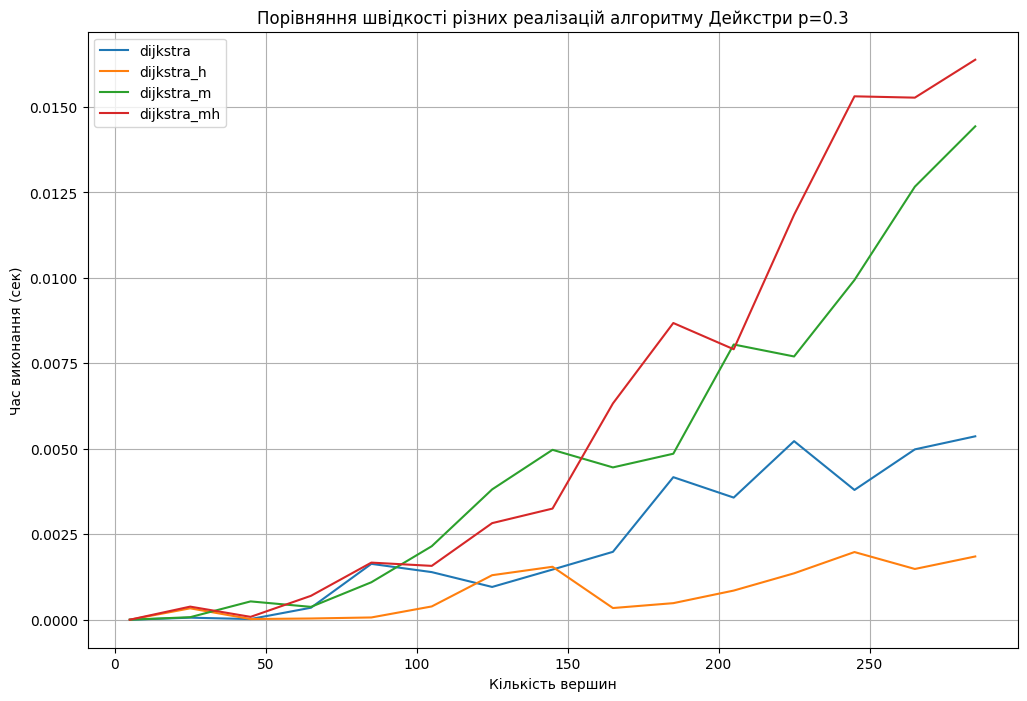
\includegraphics[width=\textwidth]{img/alldijkstra03.png}
        \caption{p=0.3}
        \label{fig:alldijkstra03}
    \end{minipage}
    \hfill
    \begin{minipage}{0.45\textwidth}
        \centering
        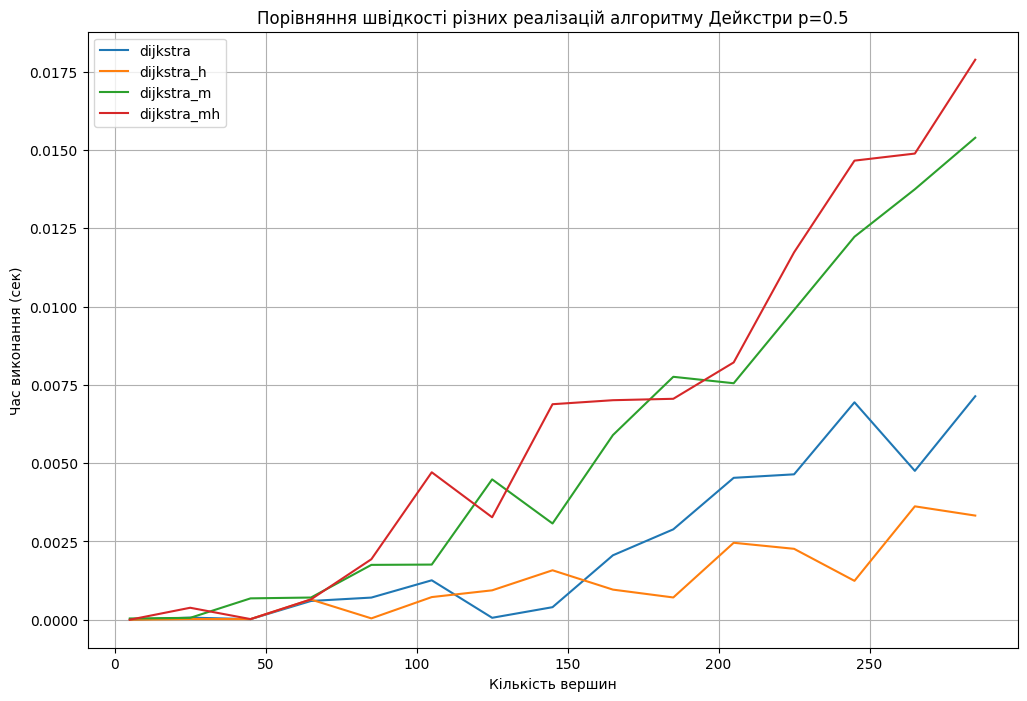
\includegraphics[width=\textwidth]{img/alldijkstra05.png}
        \caption{p=0.5}
        \label{fig:alldijkstra05}
    \end{minipage}
    
    
    \vspace{10pt} 
    \begin{minipage}{0.45\textwidth}
        \centering
        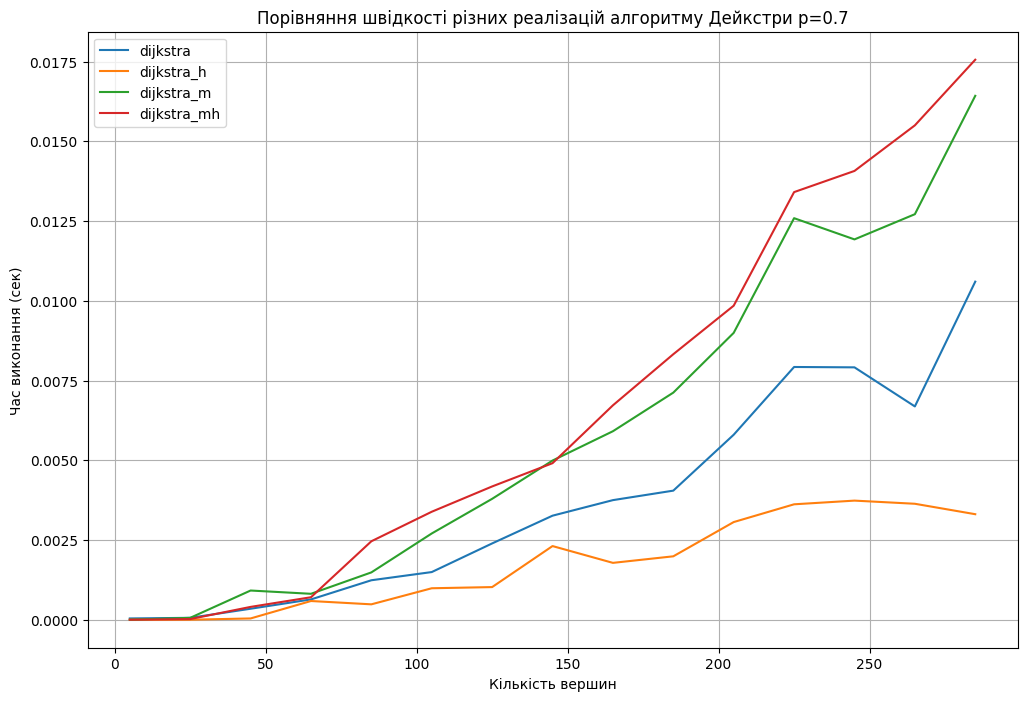
\includegraphics[width=\textwidth]{img/alldijkstra07.png}
        \caption{p=0.7}
        \label{fig:alldijkstra07}
    \end{minipage}

    Для кожної кількості вершин було проведено 50 ітерацій і взято середнє значення. Як бачимо, не зважаючи на щільність чи кількість вершин, в будь якому випадку швидкості йдуть як: 
    dijkstra\_h \textless dijkstra\_mh $\ll$ dijkstra \textless dijkstra\_m. Гіпотеза 1 підтверджена. Також підтверджено гіпотеза 2 для Дейкстри.
\end{figure}

\begin{figure}[ht]
    \centering
    \begin{minipage}{0.45\textwidth}
        \centering
        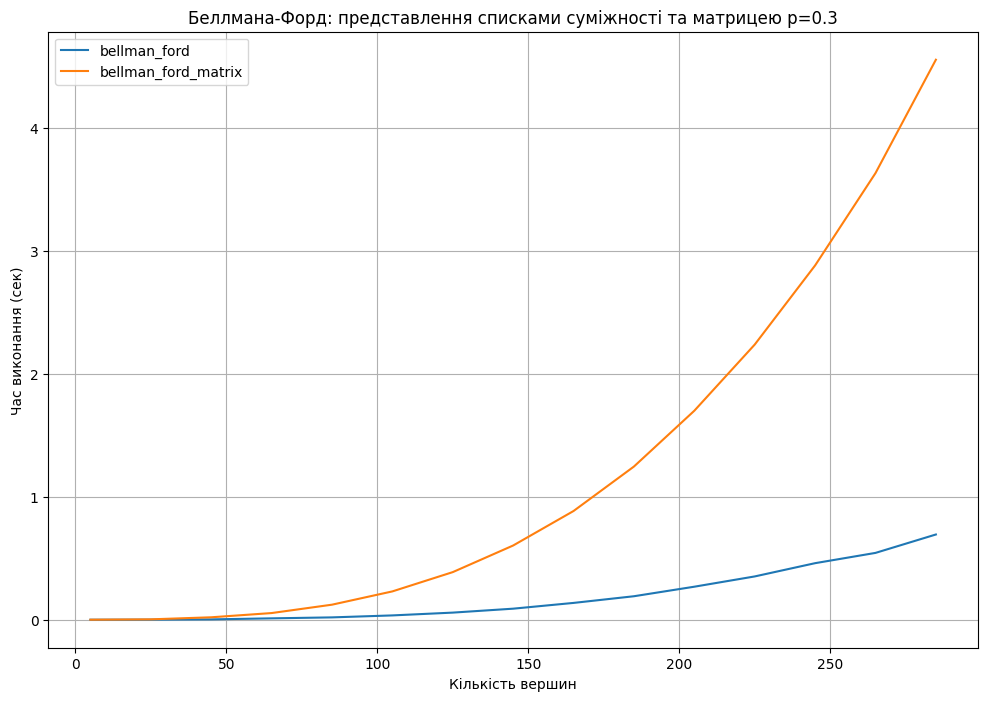
\includegraphics[width=\textwidth]{img/bellman03.png}
        \caption{p=0.3}
        \label{fig:bellman03}
    \end{minipage}
    \hfill
    \begin{minipage}{0.45\textwidth}
        \centering
        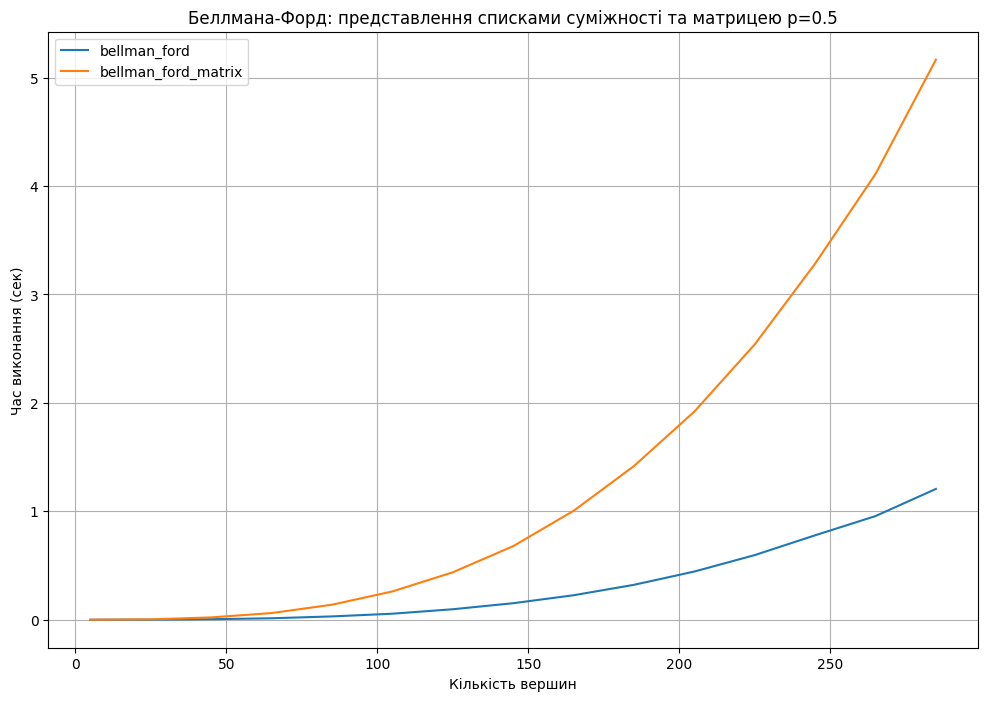
\includegraphics[width=\textwidth]{img/bellman05.png}
        \caption{p=0.5}
        \label{fig:bellman05}
    \end{minipage}
    
    
    \vspace{10pt} 
    \begin{minipage}{0.45\textwidth}
        \centering
        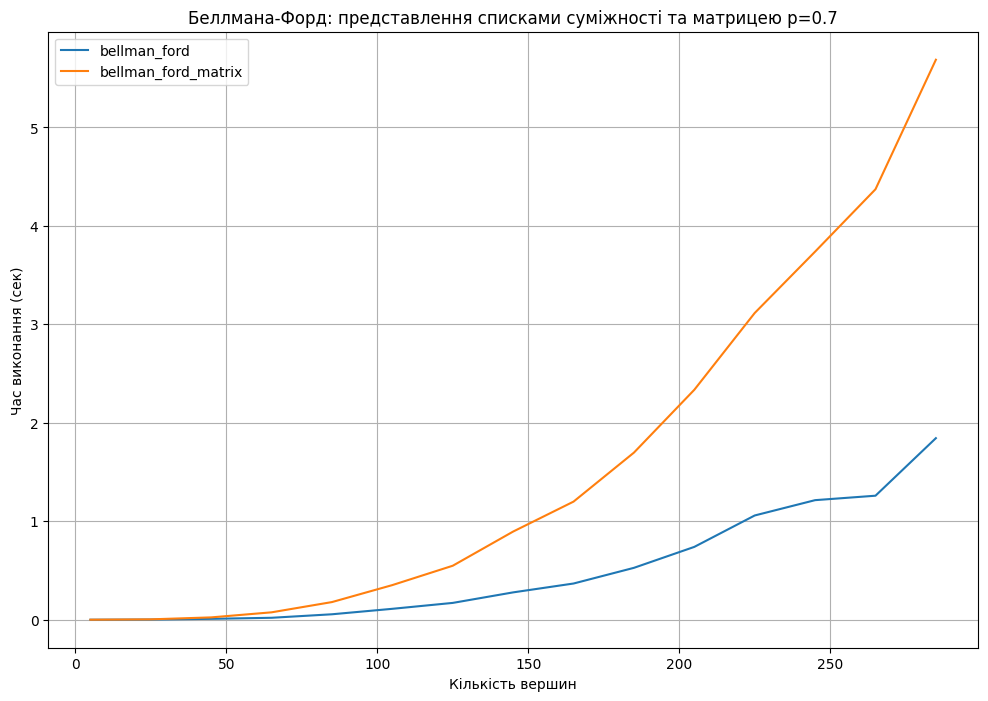
\includegraphics[width=\textwidth]{img/bellman07.png}
        \caption{p=0.7}
        \label{fig:bellman07}
    \end{minipage}
    
    Для кожної кількості вершин було проведено 50 ітерацій і взято середнє значення. Як бачимо, з ростом кількості вершин відрив представлення списками від матричного збільшується. 
    Підтверджена гіпотеза 2 для Беллмана-Форда.
\end{figure}

\begin{figure}[ht]
    \centering
    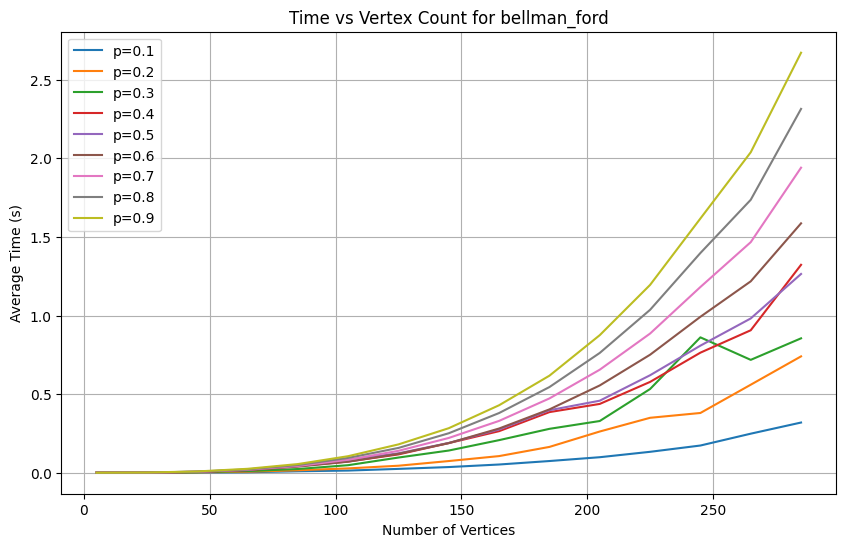
\includegraphics[width=0.8\textwidth]{img/p_bellman.png}
    \caption{Для кожної кількості вершин було проведено 100 ітерацій і взято середнє значення. Як бачимо зі збільшенням кількості вершин з'являється чітка різниця між щільностю графа: 
    зі збільшенням щільності збільшується час. Підтверджена гіпотеза 3 для Беллмана-Форда.}
    \label{fig:p_bellman}
\end{figure}

\begin{figure}[ht]
    \centering
    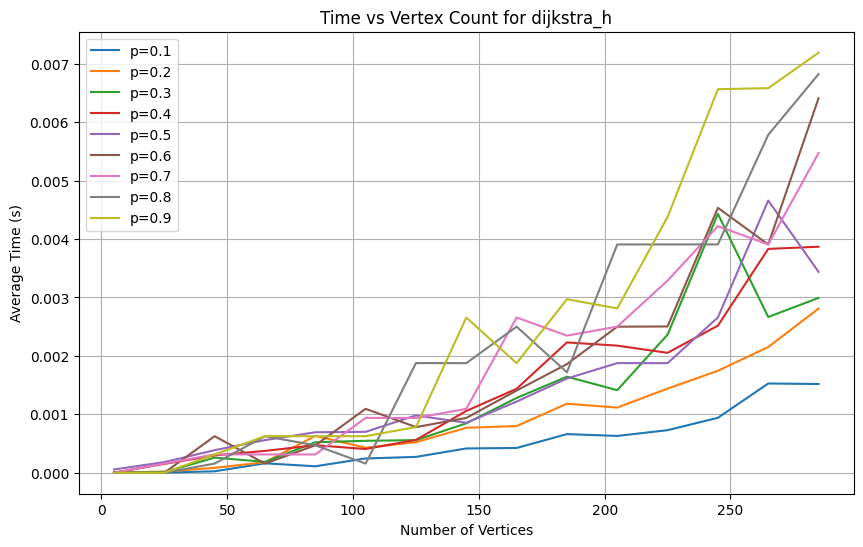
\includegraphics[width=0.8\textwidth]{img/p_dijkstra.png}
    \caption{Для кожної кількості вершин було проведено 100 ітерацій і взято середнє значення. Бачимо менш чітку різницю ніж для беллмана але вона все таки проглядається: 
    зі збільшенням щільності збільшується час роботи. Підтверджена гіпотеза 3 для Дейкстри.}
    \label{fig:p_dijkstra}
\end{figure}


\begin{figure}[ht]
    \centering
    \begin{minipage}{0.45\textwidth}
        \centering
        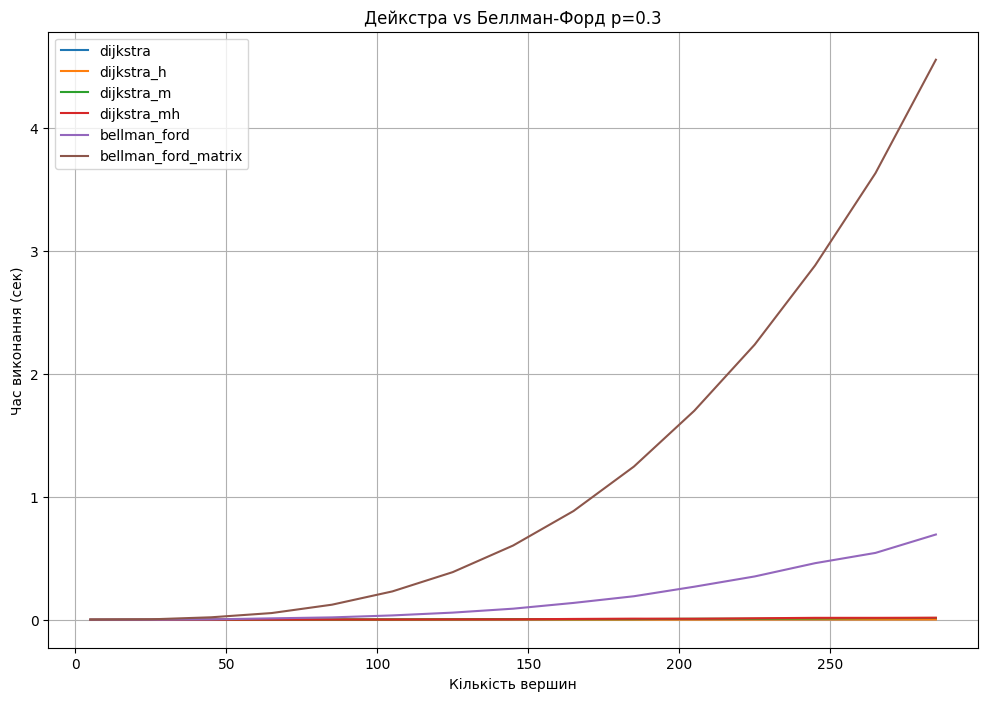
\includegraphics[width=\textwidth]{img/all03.png}
        \caption{p=0.3}
        \label{fig:all03}
    \end{minipage}
    \hfill
    \begin{minipage}{0.45\textwidth}
        \centering
        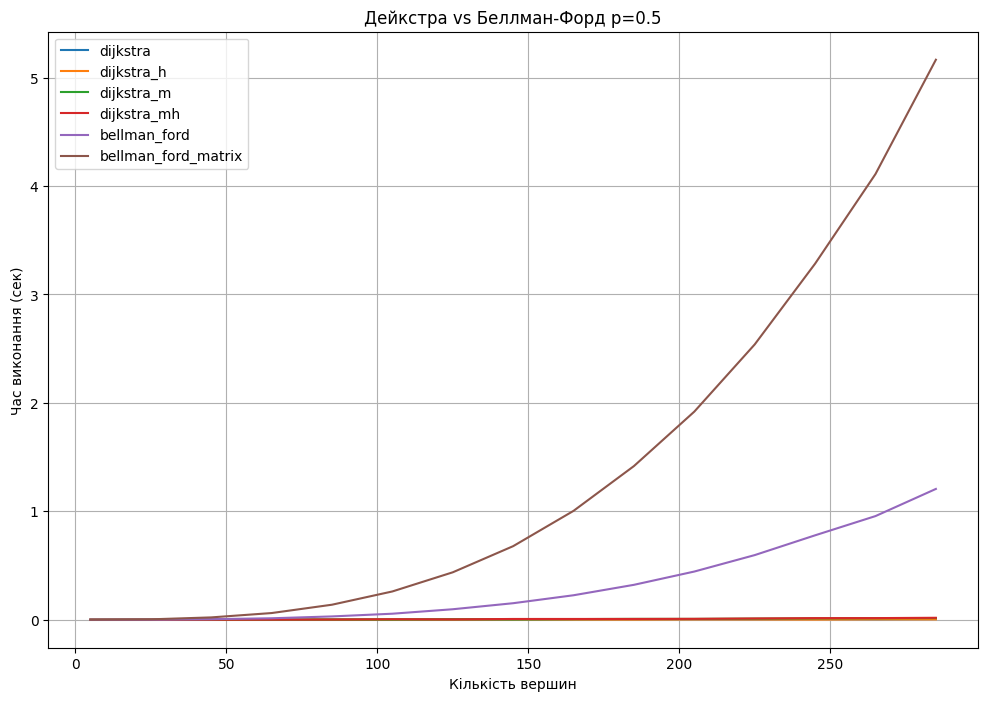
\includegraphics[width=\textwidth]{img/all05.png}
        \caption{p=0.5}
        \label{fig:all05}
    \end{minipage}
    
    
    \vspace{10pt} 
    \begin{minipage}{0.45\textwidth}
        \centering
        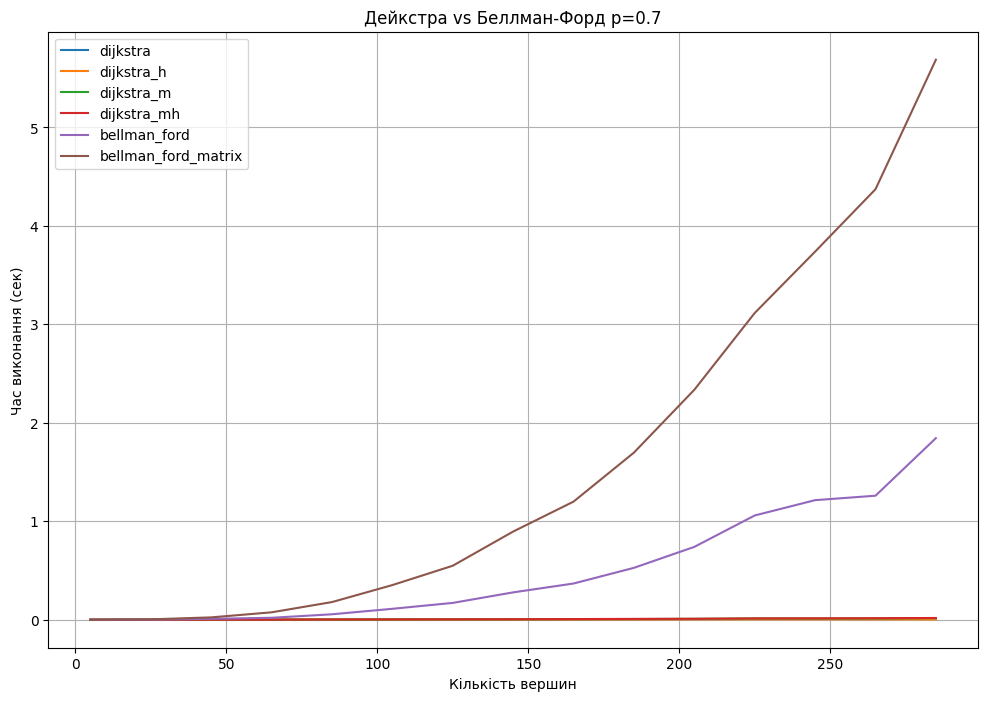
\includegraphics[width=\textwidth]{img/all07.png}
        \caption{p=0.7}
        \label{fig:all07}
    \end{minipage}

    Для кожної кількості вершин було проведено 50 ітерацій і взято середнє значення. Як бачимо, не зважаючи на щільність чи кількість вершин, в будь якому випадку час 
    Дейкстри набагато менше ніж Беллмана-Форда. Підтверджено гіпотезу 4.
\end{figure}
\clearpage
\section{Висновок}
У цій лабораторній роботі були реалізовані алгоритми Дейкстри та Беллмана-Форда для пошуку шляхів найменшої ваги в графі. 
Результати показали, що найкраще для цих алгоритмів граф представлений у вигляді списків суміжності. Алгоритм Дейкстри значно швидше Беллмана-Форда. 
Єдиним плюсом алгоритму Беллмана-Форда є його вміння працювати з від'ємними вагами ребер.
Для більш детальної інформації, будь ласка, відвідайте наступний ресурс:
\href{https://github.com/gre1wy/AppliedAlgorithms/tree/main/lab3}{Перейти до репозиторію}.

\end{document}